\documentclass[openany]{article}

%Typesetting and language
\usepackage[american]{babel}
\usepackage[T1]{fontenc}
\usepackage{charter}
\usepackage{enumitem}
\usepackage{hyperref}

%Symbols
\usepackage{amssymb, amsmath, amsthm, bm}
\usepackage{mathrsfs}
\usepackage{mathtools}
\usepackage{marvosym}
\usepackage{MnSymbol}

%Colors & graphics
\usepackage[dvipsnames]{xcolor}
\usepackage{pgfplots}
\usepackage[numbered,framed]{matlab-prettifier}
\usepackage{pgfplots}
\usepackage{listings}
\usepackage{tikz}
\usetikzlibrary{arrows.meta}
\usepackage[object=vectorian]{pgfornament}
\usepackage{wrapfig}
\usepackage{varwidth}
\usepackage[framemethod=TikZ]{mdframed}
\usepackage{caption}
\usepackage{float}
\usepackage{geometry}
\usepackage{ulem}
\usepackage[most]{tcolorbox}
\usepackage{array}

\setlength{\parindent}{0pt}

\makeatletter
\g@addto@macro\bfseries{\boldmath}
\makeatother


\renewcommand{\Re}{\mathfrak{Re}}
\renewcommand{\Im}{\mathfrak{Im}}

\geometry{left=2cm,right=2cm,bottom=2cm,top=2cm}

\usepackage{fancyhdr}
\pagestyle{fancy}
\fancyhf{}
\renewcommand{\sectionmark}[1]{\markright{\arabic{section} - #1}}
\cfoot{\thepage}
\lhead{Algo Learning}
\chead{Dynamic Programming}
\rhead{Adam Yang}
\renewcommand{\headrulewidth}{1pt}


\DeclareMathOperator{\sgn}{sgn}
\DeclareMathOperator{\im}{im}
\DeclareMathOperator{\var}{var}
\DeclareMathOperator{\Orb}{Orb}
\DeclareMathOperator{\Fix}{Fix}
\DeclareMathOperator{\Stab}{Stab}
\DeclareMathOperator{\cov}{cov}
\DeclareMathOperator*{\esssup}{ess\,sup}
\DeclareMathOperator{\corr}{corr}
\DeclareMathOperator{\lik}{lik}
\DeclareMathOperator*{\argmin}{argmin}
\DeclareMathOperator*{\argmax}{argmax}

\newcommand{\niceline}[2]{%
		\nointerlineskip \vspace{.5\baselineskip}\hspace{\fill}
		{\color{#1}
				\resizebox{0.5\linewidth}{2ex}
				{{%
								{\begin{tikzpicture}
										\node  (C) at (0,0) {};
										\node (D) at (9,0) {};
										\path (C) to [ornament=#2] (D);
										\end{tikzpicture}}}}}%
		\hspace{\fill}
		\par\nointerlineskip \vspace{.5\baselineskip}
}

\definecolor{darkViolet}{HTML}{9400D3}
\newcommand{\sweetline}{%
		\noindent
		\begin{center}
				{\color{darkViolet}
						\resizebox{0.5\linewidth}{1ex}
						{{%
										{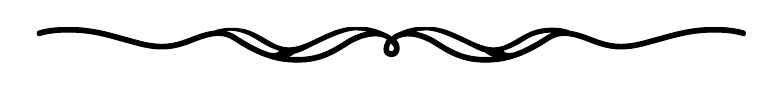
\begin{tikzpicture}
												\node  (C) at (0,0) {};
												\node (D) at (9,0) {};
												\path (C) to [ornament=85] (D);
												\end{tikzpicture}}}}}%
		\end{center}
}

\definecolor{remarkPurple}{HTML}{8346FF}
\definecolor{defBlue}{HTML}{0673FF}
\definecolor{exPurple}{HTML}{FF8710}

%THEOREM
\newtcbtheorem[auto counter,number within=section]{theorem}{Theorem}%
{enhanced,colback=white, breakable,frame empty,interior empty,colframe=cyan!50!white, top=8mm,
				coltitle=black,fonttitle=\bfseries,colbacktitle=cyan!15!white,
				borderline={0.5mm}{0mm}{cyan!15!white},
				borderline={0.5mm}{0mm}{cyan!50!white,dashed},
				attach boxed title to top left={yshift=-4mm},
				boxed title style={sharp corners=east,boxrule=1pt},varwidth boxed title}{thm}

%PROPOSITION
\newtcbtheorem[use counter from=theorem]{proposition}{Proposition}%
{enhanced,colback=white,breakable,frame empty,interior empty,colframe=defBlue!75!white, top=8mm,
				coltitle=black,fonttitle=\bfseries,colbacktitle=defBlue!20!white,
				borderline={0.5mm}{0mm}{defBlue!20!white},
				borderline={0.5mm}{0mm}{defBlue!50!white,dashed},
				attach boxed title to top left={yshift=-4mm},
				boxed title style={sharp corners=east,boxrule=1pt},varwidth boxed title}{prop}

%DEFINITION
\newtcbtheorem[use counter from=theorem]{definition}{Definition}%
{enhanced,colback=white,breakable,frame empty,interior empty,colframe=defBlue!75!white, top=8mm,
				coltitle=black,fonttitle=\bfseries,colbacktitle=defBlue!20!white,
				borderline={0.5mm}{0mm}{defBlue!20!white},
				borderline={0.5mm}{0mm}{defBlue!50!white,dashed},
				attach boxed title to top left={yshift=-4mm},
				boxed title style={sharp corners=east,boxrule=1pt},varwidth boxed title}{def}

%COROLLARY
\newtcbtheorem[use counter from=theorem]{corollary}{Corollary}%
{enhanced,colback=white,breakable,frame empty,interior empty,colframe=defBlue!75!white, top=8mm,
				coltitle=black,fonttitle=\bfseries,colbacktitle=defBlue!20!white,
				borderline={0.5mm}{0mm}{defBlue!20!white},
				borderline={0.5mm}{0mm}{defBlue!50!white,dashed},
				attach boxed title to top left={yshift=-4mm},
				boxed title style={sharp corners=east,boxrule=1pt},varwidth boxed title}{cor}

%REMARK
\newtcbtheorem[no counter]{remark}{Remark}%
{detach title, colback=white,enhanced ,breakable,frame empty, interior empty, fonttitle=\bfseries, coltitle=Violet, before upper={\tcbtitle.\quad},
				borderline west={0.5mm}{0mm}{remarkPurple!40!white},
				borderline west={0.5mm}{0mm}{remarkPurple!60!white,dashed}}{remark}

%LEMMA
\makeatletter
\newtcbtheorem[number within = tcb@cnt@theorem]{lemma}{Lemma}%
{enhanced,breakable,colback=white,frame empty,interior empty,colframe=orange!75!white, top=8mm,
				coltitle=black,fonttitle=\bfseries,colbacktitle=orange!20!white,
				borderline={0.5mm}{0mm}{orange!20!white},
				borderline={0.5mm}{0mm}{orange!50!white,dashed},
				attach boxed title to top left={yshift=-4mm},
				boxed title style={sharp corners=east,boxrule=1pt},varwidth boxed title}{lemma}
\makeatother


%PROOF
%%{enhanced,breakable,frame empty,interior empty,colframe=remarkPurple!75!white, top=8mm,
%	coltitle=black,fonttitle=\bfseries,colbacktitle=remarkPurple!20!white,
%	borderline={0.5mm}{0mm}{remarkPurple!20!white},
%	borderline={0.5mm}{0mm}{remarkPurple!50!white,dashed},
%	attach boxed title to top left={yshift=-4mm},
%	boxed title style={sharp corners=east,boxrule=1pt},varwidth boxed title}{prf}


\tcolorboxenvironment{proof}{% amsthm' 
				blanker,breakable,left=5mm,
				before skip=10pt,after skip=10pt,
				borderline west={0.5mm}{0pt}{cyan!40},
				borderline west={0.5mm}{0pt}{remarkPurple!10, dashed}}

%PROBLEM
\newtcbtheorem[auto counter]{problem}{Problem}%
{enhanced,breakable,colback=white,frame empty,interior empty,colframe=cyan!50!white, top=8mm,
				coltitle=black,fonttitle=\bfseries,colbacktitle=cyan!20!white,
				borderline={0.5mm}{0mm}{cyan!20!white},
				borderline={0.5mm}{0mm}{cyan!50!white,dashed},
				attach boxed title to top left={yshift=-4mm},
				boxed title style={sharp corners=east,boxrule=1pt},varwidth boxed title}{prob}

%EXAMPLE
%\newtcbtheorem[use counter from=problem]{example}{Example}%
%{enhanced,breakable,colback=white,frame empty,interior empty,colframe=remarkPurple!50!white, top=8mm,
%		coltitle=black,fonttitle=\bfseries,colbacktitle=remarkPurple!30!white,
%		borderline={0.5mm}{0mm}{remarkPurple!30!white},
%		borderline={0.5mm}{0mm}{remarkPurple!30!white,dashed},
%		attach boxed title to top left={yshift=-4mm},
%		boxed title style={sharp corners=east,boxrule=1pt},varwidth boxed title}{ex}


\newtcbtheorem[use counter from=theorem]{example}{Example}%
{detach title, colback=white,enhanced ,breakable,frame empty, interior empty, fonttitle=\bfseries, coltitle=black, before upper={\tcbtitle.\quad},
		borderline west={0.5mm}{0mm}{remarkPurple!30!white},
		borderline ={0.5mm}{0mm}{remarkPurple!30!white}}{example}

%SOLUTION
\newtcbtheorem[no counter]{solution}{Solution}%
{enhanced,breakable,colback=white,frame empty,interior empty,colframe=green!75!white, top=8mm,
				coltitle=black,fonttitle=\bfseries,colbacktitle=green!20!white,
				borderline={0.5mm}{0mm}{green!20!white},
				borderline={0.5mm}{0mm}{green!50!white,dashed},
				attach boxed title to top left={yshift=-4mm},
				boxed title style={sharp corners=east,boxrule=1pt},varwidth boxed title}{sol}
\definecolor{realPurple}{HTML}{AA05F9}
\definecolor{gray}{rgb}{0.5,0.5,0.5}
\definecolor{dkgreen}{rgb}{0,0.6,0}
\definecolor{mauve}{rgb}{0.58,0,0.82}

\lstset{frame=tb,
				style=Matlab-editor,
				language=C,
				aboveskip=3mm,
				belowskip=3mm,
				xleftmargin=3mm,
				showstringspaces=false,
				columns=flexible,
				frame=none,
				basicstyle={\small\ttfamily},
				numberstyle=\tiny\color{gray},
				keywordstyle=\color{blue},
				commentstyle=\color{dkgreen},
				stringstyle=\color{mauve},
				breaklines=true,
				breakatwhitespace=true,
				mlshowsectionrules = true,
				tabsize=3,
				backgroundcolor=\color{cyan!5}
}

\newcommand\mmybox[2][fill=cyan!20]{%
    \tikz[baseline]\node[%
        inner ysep=0pt, 
        inner xsep=2pt, 
        anchor=text, 
        rectangle, 
        rounded corners=1mm,
        #1] {\strut#2};%
}


\def\changemargin#1#2{\list{}{\rightmargin#2\leftmargin#1}\item[]}
\let\endchangemargin=\endlist

\linespread{1.4}



% MAIN DOC
\begin{document}

\title{Dynamic Programming}
\author{Adam Yang}
% \date{\today}
\maketitle




\section*{Problem1}

\subsection*{Algorithm}
\begin{proof}[Algorithm]{}
		\renewcommand{\qedsymbol}{}
		An Algorithm to calculate the sequence of die rolls gets to winning square as quickly as possible.
		\begin{lstlisting}[basicstyle=\fontsize{8}{9}\selectfont\ttfamily]
// this is a pseudo-code, for convenience we define add_roll() for vector<T> similar to push_back() in C++. It returns an original list added with a new square at the end and won't impact original list
// push_back() is simply C++ push_back() method for vector<T>

vector<int> findSeq( int[] d ) //d[] is the input array of information
{
    // define infinity as the largest number we can get
    // define {infinity}.size() = infinity
    // won't use INT_MAX for convenience (overflowing issue)
    // here we denote the size of d[] as n
    // if i is a ladder, d[i] = j, j>i (j is the termination of i)
    // if i is a chute, d[i] = infinity
    // if i is a normal square, d[i] = i
    // Will explain the code later
    if(n <= 6) return {n}; //trivially solved by rolling once to n
    vector<vector<int>> dp({}, n+1);
    //initialization
    for(int i = n-1; i >= n-6; --i){
        dp[i] = {n-i};
    }
    // start finding sequence
    for(int i = n-7; i >= 0; --i) {
        int min_index = -1;
        vector<int> min_seq = {infinity};
        // for some i, if d[i] = infinity, dp[infinity] = {infinity}
        // OPT(i) = min( 1 + OPT(d[i+r]) ), r = 1,2,...,6
        for(int s = i+1; s <= i+6; ++s){
            if(dp[d[s]].size() < min_seq.size()){
                min_index = s;
                min_seq = dp[d[s]];
            }
        }
        if(min_index == -1) {   //i+1:i+6 are all chute
            dp[i] = {infinity}
        } else {
            dp[i] = min_seq.add_roll(min_index - i) // sequence is reverse now, will reverse later
        }
    }
    return dp[0].reverse(); //if dp[n].size() == infinity, we can't reach n
}
		\end{lstlisting} 
\end{proof}



\begin{proof}[Explanation]{}
		\renewcommand{\qedsymbol}{} % hide the QED square
        I'll explain some variable used in pseudo-code above here

        \textbf{int[] d:} this is an input array that the problem provides, d[i] stores the information for each square, as explained from line 3 to 7
        
        \textbf{vector<vector<int>> dp:} this array needs n+1 elements since the map ranges from 0 to n. i $\in$ [0 , n], dp[i] stores the sequence with fewest times of rolls to reach n starting from i. (Prove later)
        
        \textbf{vector<T>.add\_roll():} this method add the new roll to the original vector. Return value and its general implementation is discussed in line 1.
        
        \textbf{return dp[0].reverse()} Since we always add a new roll to the end of the vector on line 30, we need to reverse to return a correct-order sequence
        
        \textit{Initialization:} \textbf{dp[n] = \{\}} because it takes no effort to reach n from n. \textbf{For i=n-6, n-5,..., n-1} we initialize dp[i] = \{n-i\} since we can reach n from i by rolling n-i = 1,2,...,6 once.

       
\end{proof}

\subsection*{Proof}
\begin{proof}[Correctness]{}
    For convenience, saying a sequence S is better than S' for square i means S takes less times of rolls to reach n than S' takes (|S| < |S'|). Optimal sequence of i means this sequence takes fewest times of rolls to reach n starting from i (i could be anything and won't matter since we start from i)
    
\textbf{Goal:} Find the optimum sequence of roll to reach n starting from 0.

\textbf{Explanation:} Starting from i, we can roll once to reach i+s, s=1,2,...,6. Denotes (i+s)'s destination by d[i+s], d[i+s]$\geq$i+s>i. Incur the sequence of (i+s) and d[i+s] to be *optimal*. The optimum does the best of six.
    
\textbf{Subproblem:}
    Starting from i, find the optimal sequence to reach n.
    
\textbf{Define:} Opt(i) to be the least times of roll to reach n starting from i. Define Opt($\infty$) := $\infty$ since there is no way to reach n.
    
\textbf{Recurrence Relation:}
    \texttt{Opt(i) = $\min_{s=1,2,...,6}$(1 + Opt( d[i+s] ) )}
    Notice that it is Opt(d[i+s]) instead of Opt(i+s). This is because i+s may be a chute, a ladder, or a normal square and d[i+s] can take their properties into consideration. If it is a chute, d[i+s] = $\infty$ > countable integer, meaning we won't choose to roll to a chute. If for some i$\in$[0,n-7], $\forall s = 1,2,...,6: $d[i+s] = $\infty$, there is no way i could be a start point to reach n, thus Opt(i) = $\infty$. If it is not, we will find the smallest of the Opt(d[i+s]) and add an additional roll to reach (i+s).
    
\textbf{Base Case:}
    \texttt{Opt(n) = 0, Opt(n-s) = 1, s = 1,2,...,6}
    
\textbf{Correctness Proof:}

    \textbf{To Prove:} dp[0].size() = Opt(0)
    
    We'll prove by strong induction of n-k, k = n, n-1, n-2, ..., 0, n-k = 0,1,2,...,n
    
    \textbf{Base Case:} dp[n].size() = Opt(n) = 0; dp[n-1].size() = dp[n-2].size() = ... = dp[n-6].size() = Opt(n-1) = Opt(n-2) = ... = Opt(n-6)
    
    \textbf{Inductive Hypothesis:} for n-k $\leq$ n-1, dp[k] = Opt(k), 0<k$\leq$n-1
    
    \textbf{Inductive Step:} when n-k = n $\Rightarrow$ k = 0, the algorithm leads to (Although the algorithm assigns vector sequence to find the sequence, since the times of rolls can be easily find through *.size()* method, finding the min times of rolls equals finding the optimal sequence)
    \begin{center}
        \texttt{dp[0].size() = min$_{s=1,2,...,6}$( 1+ dp[ d[0+s] ].size() ) = min$_{s=1,2,...,6}$( 1+ Opt( d[0+s] ) )}
    \end{center}
    [by IH, because s=1,2,...,6: n-(k+s) $\leq$ n-1 when k = 0]
    Therefore,
    \begin{center}
        \texttt{dp[0].size() = Opt(0)} [by Recurrence Relation]
    \end{center}
    
    So we find the min times of rolls to reach n from 0, and therefore the optimal sequence. If min times is $\infty$, we can't reach n. This completes the proof.

\end{proof}

\subsection*{Running Time}
\begin{proof}[Running Time]{Analyze the algorithm running time}
    	\renewcommand{\qedsymbol}{}
    	From line 14-19, setting variables and assignment takes $\mathcal{O}(n)$ for the vector. From line 21 to 37, it takes $\mathcal{O}(n)$ for looping n-6 elements and $\mathcal{O}(1)$ assignment inside (line 26 to 31 simply find the smallest times of rolls among six elements, it takes $\mathcal{O}(1)$ for six elements).
    	
    	Thus the running time $T(n)$ will be \[T(n)=2\mathcal{O}(n)=\mathcal{O}(n)\]
\end{proof}

\section*{Problem 2}





% END MAIN Doc
\end{document}
